\chapter{Time series models}\label{chap8}
In this chapter, we provide a brief introduction to performing inference in time series models using a Bayesian framework. There is a large literature in time series in statistics and econometrics, and it would be impossible to present a good treatment in a few pages of an introductory book. However, there are excellent books in Bayesian inference in time series, see for instance, \cite{west2006bayesian,petris2009dynamic,pole2018applied}.

A time series is a sequence of observations collected in chronological order, allowing us to track how variables change over time. However, it also introduces technical challenges, as we must account for statistical features such as autocorrelation and stationarity. Since time series data is time-dependent, we adjust our notation. Specifically, we use $t$ and $T$ instead of $i$ and $N$ to explicitly indicate time.

Our starting point in this chapter is the \textit{state-space representation} of time series models. Much of the Bayesian inference literature in time series adopts this approach, as it allows dynamic systems to be modeled in a structured way. This representation provides modularity, flexibility, efficiency, and interpretability in complex models where the state evolves over time. It also enables the use of recursive estimation methods, such as the \textit{Kalman filter} for dynamic Gaussian linear models and the \textit{particle filter} (also known as \textit{sequential Monte Carlo}) for non-Gaussian and nonlinear state-space models. The latter method is especially useful for \textit{online} predictions or when there are data storage limitations. These inferential tools are based on the sequential updating process of Bayes' rule, where the posterior at time $t$ becomes the prior at time $t+1$ (see Equation \ref{equpdate}).

Remember that we can run our GUI typing

\begin{tcolorbox}[enhanced,width=4.67in,center upper,
	fontupper=\large\bfseries,drop shadow southwest,sharp corners]
	\textit{R code. How to display our graphical user interface}
	\begin{VF}
		\begin{lstlisting}[language=R]
		shiny::runGitHub("besmarter/BSTApp", launch.browser = T)\end{lstlisting}
	\end{VF}
\end{tcolorbox} 

in the \textbf{R} package console or any \textbf{R} code editor, and once our GUI is deployed, select \textit{Time series Models}. However, users should see Chapter \ref{chapGUI} for details.

\section{State-space representation}\label{sec81}
A \textit{state-space model} is composed by of an \textit{unobservable state vector}  $\bm{\beta}_t \in \mathbb{R}^K$, and an \textit{observed} measure $\bm{Y}_t \in \mathbb{R}^M$, $t=1,2,\dots$ such that (i) $\bm{\beta}_t$ is a \textit{Markov process}, this is, $\pi(\bm{\beta}_t|\bm{\beta}_{1:t-1})=\pi(\bm{\beta}_t|\bm{\beta}_{t-1})$, all the information regarding $\bm{\beta}_t$ based on all its history up to $t-1$ is carried by $\bm{\beta}_{t-1}$, and (ii) $\bm{Y}_t$ is independent of $\bm{Y}_s$ conditional on $\bm{\beta}_t$, $t\neq s$ \cite[Chap.~2]{petris2009dynamic}.

These assumptions imply that $\pi(\bm{\beta}_{0:t},\bm{Y}_{1:t})=\pi(\bm{\beta}_0)\prod_{s=1}^{t}\pi(\bm{\beta}_s|\bm{\beta}_{s-1})\pi(\bm{Y}_s|\bm{\beta}_s)$.\footnote{A \textit{state-space model} where the states are random variables taking discrete values is called \textit{hidden Markov model}.}

There are three key aspects of \textit{state-space models}: \textit{filtering}, \textit{smoothing}, and \textit{forecasting}. In \textit{filtering}, we aim to estimate the current state given observations up to time $t$, specifically obtaining the density $\pi(\bm{\beta}_{s}|\bm{y}_{1:t})$ for $s = t$. In \textit{smoothing}, we conduct a retrospective analysis of the system, obtaining $\pi(\bm{\beta}_{s}|\bm{y}_{1:t})$ for $s < t$. In \textit{forecasting}, we forecast future observations by first obtaining $\pi(\bm{\beta}_{s}|\bm{y}_{1:t})$ as an intermediate step to compute $\pi(\bm{Y}_{s}|\bm{y}_{1:t})$ for $s > t$. A valuable feature of these methods is that all these densities can be calculated recursively. \cite{petris2009dynamic} show the recursive equations in Propositions 2.1 (filtering), 2.3 (smoothing) and 2.5 (forecasting).

An important class of \textit{state-space models} is the \textit{Gaussian linear state-space model}, also know as, \textit{dynamic linear model}:
\begin{align*}
	\bm{Y}_t&=\bm{X}_t\bm{\beta}_t+\bm{\mu}_t& \text{(Observation equations)}\\
	\bm{\beta}_t&=\bm{G}_t\bm{\beta}_{t-1}+\bm{w}_t & \text{(States equations)},
\end{align*}
where $\bm{\beta}_0\sim N(\bm{b}_0,\bm{B}_0)$, $\bm{\mu}_t\sim N(\bm{0}, \bm{\Sigma}_t)$, $\bm{w}_t\sim N(\bm{0}, \bm{\Omega}_t)$, $\bm{\beta}_0$, $\bm{\mu}_t$ and $\bm{w}_t$ are independent, $\bm{X}_t$ and $\bm{G}_t$ are $M\times K$ and $K\times K$ known matrices. Observe that this assumptions implies that $\bm{Y}_t|\bm{\beta}_t\sim N(\bm{X}_t\bm{\beta}_t,\bm{\Sigma}_t)$, and $\bm{\beta}_t|\bm{\beta}_{t-1}\sim N(\bm{G}_t\bm{\beta}_{t-1},\bm{\Omega}_t)$.\footnote{A general \textit{state-space model} is given by $\bm{Y}_t=\bm{f}_t(\bm{\beta}_t,\bm{\mu}_t)$, and $\bm{\beta}_t=\bm{m}_t(\bm{\beta}_{t-1},\bm{w}_t)$ for arbitrary functions $\bm{f}_t$ and $\bm{m}_t$, and distributions for $\bm{\mu}_t$ and $\bm{w}_t$, and a prior distribution for $\bm{\beta}_0$.}

Let $\bm{\beta}_{t-1}|\bm{y}_{1:t-1}\sim N(\bm{b}_{t-1},\bm{B}_{t-1})$, then, we can get the \textit{Kalman filter} by getting
\begin{enumerate}
	\item The one-step-ahead predictive distribution of $\bm{\beta}_t$ given $\bm{y}_{1:t-1}$ is $\bm{\beta}_t|\bm{y}_{1:t-1}\sim N(\bm{a}_t, \bm{R}_t)$, where $\bm{a}_t=\bm{G}_t\bm{b}_{t-1}$ and $\bm{R}_t=\bm{G}_t\bm{B}_{t-1}\bm{G}_t^{\top}+\bm{\Omega}_t$.
	\item  The one-step-ahead predictive distribution of $\bm{Y}_t$ given $\bm{y}_{1:t-1}$ is $\bm{Y}_t|\bm{y}_{1:t-1}\sim N(\bm{f}_t, \bm{Q}_t)$, where $\bm{f}_t=\bm{X}_t\bm{a}_t$ and $\bm{Q}_t=\bm{X}_t\bm{R}_t\bm{X}_t^{\top}+\bm{\Sigma}_t$.
	\item The distribution of the one-step-ahead prediction error  $\bm{e}_t=\bm{Y}_t-\mathbb{E}[\bm{Y}_t|\bm{y}_{1:t-1}]=\bm{Y}_t-\bm{f}_t$ is $N(\bm{0}, \bm{Q}_t)$ \cite[Chap.~6]{shumway2017time}. 
	\item The filtering distribution of $\bm{\beta}_t$ given $\bm{y}_{1:t}$ is $\bm{\beta}_t|\bm{y}_{1:t}\sim N(\bm{b}_t, \bm{B}_t)$, where $\bm{b}_t=\bm{a}_t+\bm{K}_t\bm{e}_t$, $\bm{K}_t=\bm{R}_t\bm{X}_t^{\top}\bm{Q}_t^{-1}$ is the \textit{Kalman gain}, and $\bm{B}_t=\bm{R}_t-\bm{R}_t\bm{X}_t^{\top}\bm{Q}_t^{-1}\bm{X}_t\bm{R}_t$.   
\end{enumerate}    

The formal proofs of these results can be found in \cite[Chap~2]{petris2009dynamic}. Just take into account that the logic of these results follow the results of the Seemingly unrelated regression (SUR) model in Section \ref{sec72} for a particular time period. In addition, we know that the posterior distribution using information up to $t-1$ becomes the prior in $t$ (see Equation \ref{equpdate}, $\pi(\bm{\theta}|\mathbf{y}_{1:t})\propto p(y_{t}|\bm{y}_{1:t-1},\bm{\theta})\times \pi(\bm{\theta}|\bm{y}_{1:t-1})$). This is the updating process from  $\bm{\beta}_t|\bm{y}_{1:t-1}\sim N(\bm{a}_t, \bm{R}_t)$ to $\bm{\beta}_t|\bm{y}_{1:t}\sim N(\bm{b}_t, \bm{B}_t)$. Moreover, the posterior mean and variance of the SUR model with independent conjugate priors for a particular time period can be written as $\bm{a}_{t}+\bm{R}_{t}\bm{X}_t^{\top}(\bm{X}_t\bm{R}_{t}\bm{X}_t^{\top}+ \bm{\Sigma}_t)^{-1}(\bm{y}_t-\bm{X}_t\bm{a}_{t})$ and $\bm{R}_{t}-\bm{R}_{t}\bm{X}_t^{\top}(\bm{X}_t\bm{R}_{t}\bm{X}_t^{\top}+\bm{\Sigma}_t)^{-1} \bm{X}_t\bm{R}_{t}^{\top}$, respectively. Let's see this, we know from Section \ref{sec72} that $\bm{B}_t=(\bm{R}_t^{-1}+\bm{X}_t^{\top}\bm{\Sigma}^{-1}\bm{X}_t)^{-1}$ and $\bm{\beta}_t=\bm{B}_t(\bm{R}_t^{-1}\bm{a}_t+\bm{X}_t^{\top}\bm{\Sigma}^{-1}\bm{y}_t)$. Thus, let's show that both conditional posterior distributions are the same. In particular, the posterior mean in the \textit{state-space representation} is $[\bm{I}_K-\bm{R}_{t}\bm{X}_t^{\top}(\bm{X}_t\bm{R}_{t}\bm{X}_t^{\top}+ \bm{\Sigma}_t)^{-1}\bm{X}_t]\bm{a}_{t}+\bm{R}_{t}\bm{X}_t^{\top}(\bm{X}_t\bm{R}_{t}\bm{X}_t^{\top}+ \bm{\Sigma}_t)^{-1}\bm{y}_t$, where 
\begin{align*}
	\bm{R}_{t}\bm{X}_t^{\top}(\bm{X}_t\bm{R}_{t}\bm{X}_t^{\top}+ \bm{\Sigma}_t)^{-1}
	&=\bm{R}_{t}\bm{X}_t^{\top}[\bm{\Sigma}_t^{-1}-\bm{\Sigma}_t^{-1}\bm{X}_t(\bm{R}_t^{-1}+\bm{X}_t^{\top}\bm{\Sigma}_t^{-1}\bm{X}_t)^{-1}\bm{X}_t^{\top}\bm{\Sigma}_t^{-1}]\\
	&=\bm{R}_{t}[\bm{I}_K-\bm{X}_t^{\top}\bm{\Sigma}_t^{-1}\bm{X}_t(\bm{R}_t^{-1}+\bm{X}_t^{\top}\bm{\Sigma}_t^{-1}\bm{X}_t)^{-1}]\bm{X}_t^{\top}\bm{\Sigma}_t^{-1}\\
	&=\bm{R}_{t}(\bm{I}_K-[\bm{I}_K-\bm{R}_t^{-1}(\bm{R}_t^{-1}+\bm{X}_t^{\top}\bm{\Sigma}_t^{-1}\bm{X}_t)^{-1}])\bm{X}_t^{\top}\bm{\Sigma}_t^{-1}\\
	&=(\bm{R}_t^{-1}+\bm{X}_t^{\top}\bm{\Sigma}_t^{-1}\bm{X}_t)^{-1}\bm{X}_t^{\top}\bm{\Sigma}_t^{-1},
\end{align*}
where the first equality uses the Woodbury matrix identity (matrix inversion lemma), and the third equality uses $\bm{D}(\bm{D}+\bm{E})^{-1}=\bm{I}-\bm{E}(\bm{D}+\bm{E})^{-1}$. 

Thus, $[\bm{I}_K-\bm{R}_{t}\bm{X}_t^{\top}(\bm{X}_t\bm{R}_{t}\bm{X}_t^{\top}+ \bm{\Sigma}_t)^{-1}\bm{X}_t]\bm{a}_{t}+\bm{R}_{t}\bm{X}_t^{\top}(\bm{X}_t\bm{R}_{t}\bm{X}_t^{\top}+ \bm{\Sigma}_t)^{-1}\bm{y}_t=[\bm{I}_K-(\bm{R}_t^{-1}+\bm{X}_t^{\top}\bm{\Sigma}_t^{-1}\bm{X}_t)^{-1}\bm{X}_t^{\top}\bm{\Sigma}_t^{-1}\bm{X}_t]\bm{a}_{t}+(\bm{R}_t^{-1}+\bm{X}_t^{\top}\bm{\Sigma}_t^{-1}\bm{X}_t)^{-1}\bm{X}_t^{\top}\bm{\Sigma}_t^{-1}\bm{y}_t=(\bm{R}_t^{-1}+\bm{X}_t^{\top}\bm{\Sigma}_t^{-1}\bm{X}_t)^{-1}\bm{R}_t^{-1}\bm{a}_{t}+(\bm{R}_t^{-1}+\bm{X}_t^{\top}\bm{\Sigma}_t^{-1}\bm{X}_t)^{-1}\bm{X}_t^{\top}\bm{\Sigma}_t^{-1}\bm{y}_t=(\bm{R}_t^{-1}+\bm{X}_t^{\top}\bm{\Sigma}_t^{-1}\bm{X}_t)^{-1}(\bm{R}_t^{-1}\bm{a}_{t}+\bm{X}_t^{\top}\bm{\Sigma}_t^{-1}\bm{y}_t)=(\bm{R}_t^{-1}+\bm{X}_t^{\top}\bm{\Sigma}_t^{-1}\bm{X}_t)^{-1}(\bm{R}_t^{-1}\bm{a}_{t}+\bm{X}_t^{\top}\bm{\Sigma}_t^{-1}\bm{X}_t\hat{\bm{\beta}}_t)$. The second equality uses $\bm{I}-(\bm{D}+\bm{E})^{-1}\bm{D}=(\bm{D}+\bm{E})^{-1}\bm{E}$, and $\hat{\bm{\beta}}_t=(\bm{X}_t^{\top}\bm{\Sigma}_t^{-1}\bm{X}_t)^{-1}\bm{X}_t^{\top}\bm{\Sigma}_t^{-1}\bm{y}_t$. This means that the posterior mean is a weighted average of the prior mean, and the maximum likelihood estimator (generalized least squares estimator).

The weights are linked to the signal-to-noise ratio, that is, the proportion of the total variability ($\bm{\Omega}_t+\bm{\Sigma}_t$) due to the signal ($\bm{\Omega}_t$) versus the noise ($\bm{\Sigma}_t$). Note that in the simplest case where $M=K=1$, and $\bm{X}_t=\bm{G}_t=1$, then $\bm{K}_t=\bm{R}_t\bm{Q}_t^{-1}=(B_{t-1}+\Omega_t)/(B_{t-1}+\Omega_t+\Sigma_t)$. Thus, the weight associated with the observations is equal to 1 if $\Sigma_t=0$, that is, the posterior mean is equal to the actual observation. On the other hand, if $\Sigma_t$ increases compare to $\Omega_t$, there is more weight to the prior information, and consequently, the posterior mean is smoother as it heavily dependents on the history. We ask in Exercise 1 to perform simulations with different signal-to-noise ratios to see the effects on the system.   

The equality of variances of both approaches is as follows:
\begin{align*}
	Var[\bm{\beta}_t|\bm{y}_{1:t}]&
	= \bm{R}_{t}-\bm{R}_{t}\bm{X}_t^{\top}(\bm{X}_t\bm{R}_{t}\bm{X}_t^\top+\bm{\Sigma}_t)^{-1} \bm{X}_t\bm{R}_{t}\\
	&=\bm{R}_{t}-\bm{R}_{t}\bm{X}_t^{\top}(\bm{\Sigma}_t^{-1}- \bm{\Sigma}_t^{-1}\bm{X}_t(\bm{R}_{t}^{-1}+\bm{X}_t^{\top}\bm{\Sigma}_t^{-1}\bm{X}_t)^{-1}\bm{X}_t^{\top}\bm{\Sigma}_t^{-1})\bm{X}_t\bm{R}_{t}\\
	&=\bm{R}_{t}-\bm{R}_{t}\bm{X}_t^{\top}\bm{\Sigma}_t^{-1}\bm{X}_t\bm{R}_{t}+ \bm{R}_{t}\bm{X}_t^{\top}\bm{\Sigma}_t^{-1}\bm{X}_t(\bm{R}_{t}^{-1}+\bm{X}_t^{\top}\bm{\Sigma}_t^{-1}\bm{X}_t)^{-1}\bm{X}_t^{\top}\bm{\Sigma}_t^{-1}\bm{X}_t\bm{R}_{t}\\
	&=\bm{R}_{t}-\bm{R}_{t}\bm{X}_t^{\top}\bm{\Sigma}_t^{-1}\bm{X}_t\bm{R}_{t}+ \bm{R}_{t}\bm{X}_t^{\top}\bm{\Sigma}_t^{-1}\bm{X}_t[\bm{I}_K-(\bm{R}_{t}^{-1}+\bm{X}_t^{\top}\bm{\Sigma}_t^{-1}\bm{X}_t)^{-1}\bm{R}_{t}^{-1}]\bm{R}_{t}\\
	&=\bm{R}_{t}-\bm{R}_{t}\bm{X}_t^{\top}\bm{\Sigma}_t^{-1}\bm{X}_t(\bm{R}_{t}^{-1}+\bm{X}_t^{\top}\bm{\Sigma}_t^{-1}\bm{X}_t)^{-1}\\
	&=\bm{R}_t[\bm{I}_K-\bm{X}_t^{\top}\bm{\Sigma}_t^{-1}\bm{X}_t(\bm{R}_{t}^{-1}+\bm{X}_t^{\top}\bm{\Sigma}_t^{-1}\bm{X}_t)^{-1}]\\
	&=\bm{R}_{t}[\bm{I}_K-(\bm{I}_K-\bm{R}_{t}^{-1}(\bm{R}_{t}^{-1}+\bm{X}_t^{\top}\bm{\Sigma}_t^{-1}\bm{X}_t)^{-1})]\\
	&=(\bm{R}_{t}^{-1}+\bm{X}_t^{\top}\bm{\Sigma}_t^{-1}\bm{X}_t)^{-1},
\end{align*}
where the second equality uses the Woodbury matrix identity, the fourth equality uses $(\bm{D}+\bm{E})^{-1}\bm{D}=\bm{I}-(\bm{D}+\bm{E})^{-1}\bm{E}$, and the seventh equality uses $\bm{D}(\bm{D}+\bm{E})^{-1}=\bm{I}-\bm{E}(\bm{D}+\bm{E})^{-1}$.  

The \textit{Kalman filter} allows calculating recursively in a forward way $\pi(\bm{\beta}_t|\bm{y}_{1:t})$ from $\pi(\bm{\beta}_{t-1}|\bm{y}_{1:t-1})$ starting from $\pi(\bm{\beta}_0)$.

Let $\bm{\beta}_{t+1}|\bm{y}_{1:T}\sim N(\bm{s}_{t+1},\bm{S}_{t+1})$, then we can get the \textit{Kalman smoother} by $\bm{\beta}_{t}|\bm{y}_{1:T}\sim N(\bm{s}_{t},\bm{S}_{t})$, where $\bm{s}_t=\bm{b}_t+\bm{B}_t\bm{G}_{t+1}^{\top}\bm{R}_{t+1}^{-1}(\bm{s}_{t+1}-\bm{a}_{t+1})$ and $\bm{S}_t=\bm{B}_t-\bm{B}_t\bm{G}_{t+1}^{\top}\bm{R}_{t+1}^{-1}(\bm{R}_{t+1}-\bm{S}_{t+1})\bm{R}_{t+1}^{-1}\bm{G}_{t+1}\bm{B}_{t}$. The proof can be found in \cite[Chap~2]{petris2009dynamic}. 

Thus, we can calculate the \textit{Kalman smoother} starting from $t=T-1$, that is, $\bm{\beta}_{T}|\bm{y}_{1:T}\sim N(\bm{s}_{T},\bm{S}_{T})$. However, this is the filtering distribution at $T$, which means $\bm{s}_{T}=\bm{b}_{T}$ and $\bm{S}_{T}=\bm{B}_{T}$, and then, we should proceed recursively in a backward way.

Finally, the forecasting recursion in the \textit{dynamic linear model}, given $\bm{a}_t(0)=\bm{b}_t$ and $\bm{R}_t(0)=\bm{B}_t$, $h\geq 1$, is given by 
\begin{enumerate}
	\item The forecasting distribution of $\bm{\beta}_{t+h}|\bm{y}_{1:t}$ is $N(\bm{a}_t(h),\bm{R}_t(h))$, where $\bm{a}_t(h)=\bm{G}_{t+h}\bm{a}_{t}(h-1)$ and $\bm{R}_t(h)=\bm{G}_{t+h}\bm{R}_t(h-1)\bm{G}_{t+h}^{\top}+\bm{\Omega}_{t+h}$.
	\item The forecasting distribution $\bm{Y}_{t+h}|\bm{y}_{1:t}$ is $N(\bm{f}_t(h),\bm{Q}_t(h))$, where $\bm{f}_t(h)=\bm{X}_{t+h}\bm{a}_t(h)$ and $\bm{Q}_t(h)=\bm{X}_{t+h}\bm{R}_t(h)\bm{X}_{t+h}^{\top}+\bm{\Sigma}_{t+h}$.  
\end{enumerate}
The proof can be found in \cite[Chap~2]{petris2009dynamic}.

These recursive equations allows to perform probabilistic forecasting $h$-steps-ahead for the state and observation equations.

These results show how to use these recursive equations to perform filtering, smoothing and forecasting in \textit{dynamic linear models} (\textit{Gaussian linear state-space models}). Despite that these algorithms look simple, they suffer from numerical instability that lead to non-symmetric and negative definite calculated covariance matrices. Thus, special care should be put when working with them.

In addition, this set up assumes that the $\bm{\Sigma}_t$ and $\bm{\Omega}_t$ are known. However, this is no the case in most situations. Thus, we should estimate them. One option is to perform maximum likelihood estimation. However, this approach does not take into account the uncertainty associated with the fact that $\bm{\Sigma}_t$ and $\bm{\Omega}_t$ are unknown when their estimates are \textit{plug in} the \textit{state space} recursions. On the other hand, we can use a Bayesian approach, and perform the recursions associated with each posterior draw of the unknown parameters. Thus, we take into account their uncertainty.

The point of departure is the posterior distribution, such that
\begin{align*}
	\pi(\bm{\theta},\bm{\beta}_0,\dots,\bm{\beta}_T|\bm{y}, \bm{X}, \bm{G})&\propto\pi(\bm{\beta}_0|\bm{\theta})\pi(\bm{\theta})\prod_{t=1}^{T}\pi(\bm{\beta}_t|\bm{\beta}_{t-1},\bm{\theta})\pi(\bm{y}_t|\bm{\beta}_t,\bm{\theta}),
\end{align*} 
where $\bm{\theta}$ is the vector of unknown parameters.

We can compute $\pi(\bm{\beta}_s,\bm{\theta}|\bm{y}_{1:t})=\pi(\bm{\beta}_s|\bm{y}_{1:t},\bm{\theta})\pi(\bm{\theta}|\bm{y}_{1:t})$, for $s=t$ (\textit{filtering}), $s<t$ (\textit{smoothing}), and $s>t$ (\textit{forecasting}). The marginal posterior distribution of the states is $\pi(\bm{\beta}_s|\bm{y}_{1:t})=\int_{\bm{\Theta}}\pi(\bm{\beta}_s|\bm{y}_{1:t},\bm{\theta})\pi(\bm{\theta}|\bm{y}_{1:t})d\bm{\theta}$.

We can use the Gibbs sampling algorithm to get the posterior draws in the \textit{dynamic linear model} assuming conjugate families. In particular, let's see the univariate case with \textit{random walk states}, 
\begin{align}
	Y_t&=\bm{x}_t^{\top}\bm{\beta}_t+\mu_t\label{eq1Obs}\\
	\bm{\beta}_t&=\bm{\beta}_{t-1}+\bm{w}_t \label{eq1St},
\end{align}
where $\mu_t\sim N(0,\sigma^2)$ and $\bm{w}_t\sim N(\bm{0},\text{diag}\left\{\omega_1^2,\dots,\omega_K^2\right\})$. We assume that $\pi(\sigma^2,\omega_1^2,\dots,\omega_K^2,\bm{\beta}_0)=\pi(\sigma^2)\pi(\omega_1^2),\dots,\pi(\omega_K^2)\pi(\bm{\beta}_0)$ where $\sigma^2\sim IG(\alpha_0/2,\delta_0/2)$, $\omega_k^2\sim IG(\alpha_{k0}/2,\delta_{k0}/2)$, $k=1,\dots,K$, and $\bm{\beta}_0\sim N(\bm{b}_0,\bm{B}_0)$. Thus, the conditional posterior distributions are $\sigma^2|\bm{y},\bm{X},\bm{\beta}_{1:T}\sim IG(\alpha_{n}/2,\delta_n/2)$, where $\alpha_{n}=T+\alpha_0$ and $\delta_n=\sum_{t=1}^T(y_t-\bm{x}_t^{\top}\bm{\beta}_t)^2+\delta_0$, and $\omega_k^2|\bm{y},\bm{X},\bm{\beta}_{0:T}\sim IG(\alpha_{kn}/2,\delta_{kn}/2)$, where $\alpha_{kn}=T+\alpha_{k0}$ and $\delta_{kn}=\sum_{t=1}^T(\bm{\beta}_{t,k}-\bm{\beta}_{t-1,k})^2+\delta_{k0}$. The vector of the dependent variable is $\bm{y}$, and all regressors are in $\bm{X}$.

We also need to sample the states from $\pi(\bm{\beta}_{1:T}|\bm{y},\bm{X},\sigma^2,\omega_1^2,\dots,\omega_K^2)$. This can be done using the forward filtering backward sampling (FFBS) algorithm \cite{carter1994gibbs,fruhwirth1994data,shephard1994partial}. This algorithm is basically a simulation version of the \textit{smoothing} recursion, which allows getting draws of the states, even if we do not have analytical solutions, for instance, in non-linear settings. See below and \cite[Chap.~3]{petris2009dynamic} for details. A word of caution here, users should be careful to set non-informative priors in this setting, and in general, settings where there are a large number of parameters (see \cite[Chap.~8]{koop2003bayesian} for details). Thus, it is useful to use empirical Bayes methods focusing on relevant hyperparameters, for instance, the hyperparameters of the inverse-gamma distributions which define the signal-to-noise ratio.   

We use the command \textit{dlmGibbsDIG} from the \textit{dlm} package in our GUI to perform Bayesian inference in the univariate \textit{dynamic linear model} with \textit{random walk states}. This function uses the FFBS algorithm, and assumes independent inverse-gamma priors for the scale parameters. In addition, this package uses the singular value decomposition to calculate the covariance matrices to avoid numerical instability.

Algorithm \ref{alg:DLM} shows how to perform inference in univariate \textit{dynamic linear model} with random walk states in our GUI. See also Chapter \ref{chapGUI} for details regarding the dataset structure.

\begin{algorithm}[h!]
	\caption{Dynamic linear models}\label{alg:DLM}
	\begin{algorithmic}[1]  		 			
		\State Select \textit{Time series Model} on the top panel
		\State Select \textit{Dynamic linear model} using the left radio button
		\State Upload the dataset selecting first if there is header in the file, and the kind of separator in the \textit{csv} file of the dataset (comma, semicolon, or tab). Then, use the \textit{Browse} button under the \textbf{Choose File} legend
		\State Select MCMC iterations, burn-in and thinning parameters using the \textit{Range sliders}
		\State Set the hyperparameters of the \textit{variance of the observation equation}: prior mean and variance. This step is not necessary as by default our GUI uses non-informative priors
		\State Set the hyperparameters of the \textit{variance of the state equations}: just one set of prior mean and variance parameters. This step is not necessary as by default our GUI uses non-informative priors
		\State Click the \textit{Go!} button
		\State Analyze results
		\State Download posterior chains and diagnostic plots using the \textit{Download Posterior Chains} and \textit{Download Posterior Graphs} buttons
	\end{algorithmic} 
\end{algorithm}

\textbf{Example: Simulation exercise of the dynamic linear model}

We simulate the process $y_t=\beta_{t1}+{x}_t{\beta}_{t2}+\mu_t$ and $\bm{\beta}_t=\bm{\beta}_{t-1}+\bm{w}_t$, $t=1,2,\dots,200$, where $\bm{\beta}_t=[\beta_{t1} \ {\beta}_{t2}]^{\top}$, $\mu_t\sim N(0,0.5^2)$, $\bm{w}_t\sim N(\bm{0},\text{diag}\left\{0.2,0.1\right\})$, $x_t\sim N(1, 1)$, $\bm{\beta}_0$ and $\bm{B}_0$ are the OLS estimates and variance of the recursive OLS estimates (see below), respectively.

The following algorithm shows how to perform inference using \textit{dlmGibbsDIG}, and compares the results to the maximum likelihood estimator. The latter is based on \textit{dlmMLE} function. We also use the \textit{dlmSvd2var} function, that is based on the singular value decomposition, to calculate the variance of the smoothing states.

Users can observe that we employ a straightforward strategy for setting the hyperparameters. First, we recursively estimate the model using ordinary least squares (OLS), progressively increasing the sample size, and save the location parameters. Next, we compute the covariance matrix of this sequence and use it to set the priors: the prior mean of the state vector variance is set to the maximum element of the main diagonal of this covariance matrix (\textit{a.theta}), and the prior variance is set to ten times this value (\textit{b.theta}). For the observation equation, the prior mean of the variance is set to the OLS estimate (\textit{a.y}), and the prior variance is set to ten times this value (\textit{b.y}). We perform some sensitivity analysis of the results regarding the hyperparameters, and it seems that the results are robust. However, we encourage to give more consideration to empirical Bayes methods for setting hyperparameters in \textit{state-space models}.

\begin{tcolorbox}[enhanced,width=4.67in,center upper,
	fontupper=\large\bfseries,drop shadow southwest,sharp corners]
	\textit{R code. Simulation: Dynamic linear model}
	\begin{VF}
		\begin{lstlisting}[language=R]
rm(list = ls()); set.seed(010101)
T <- 200; sig2 <- 0.5^2
x <- rnorm(T, mean = 1, sd = 1) 
X <- cbind(1, x); B0 <- c(1, 0.5)
K <- length(B0)
e <- rnorm(T, mean = 0, sd = sig2^0.5)
Omega <- diag(c(0.2, 0.1))
w <- MASS::mvrnorm(T, c(0, 0), Omega)
Bt <- matrix(NA, T, K); Bt[1,] <- B0
yt <- rep(NA, T) 
yt[1] <- X[1,]%*%B0 + e[1]
yt[1] <- x[1]*Bt[1] + e[1]
for(t in 1:T){
	if(t == 1){
		Bt[t,] <- w[t,]
	}else{
		Bt[t,] <- Bt[t-1,] + w[t,]
	}
	yt[t] <- X[t,]%*%Bt[t,] + e[t]
}
RegLS <- lm(yt ~ x)
SumRegLS <- summary(RegLS)
SumRegLS; SumRegLS$sigma^2  
Bp <- matrix(RegLS$coefficients, T, K, byrow = TRUE)
S <- 20
for(t in S:T){
	RegLSt <- lm(yt[1:t] ~ x[1:t])
	Bp[t,] <- RegLSt$coefficients 
}
# plot(Bp[S:T,2], type = "l")
VarBp <- var(Bp)
# State spece model
ModelReg <- function(par){
	Mod <- dlm::dlmModReg(x, dV = exp(par[1]), dW = exp(par[2:3]), m0 = RegLS$coefficients,	C0 = VarBp)
	return(Mod)
}
outMLEReg <- dlm::dlmMLE(yt, parm = rep(0, K+1), ModelReg)
exp(outMLEReg$par)
RegFilter <- dlm::dlmFilter(yt, ModelReg(outMLEReg$par))
RegSmoth <- dlm::dlmSmooth(yt, ModelReg(outMLEReg$par))
SmoothB2 <- RegSmoth$s[-1,2]
VarSmooth <- dlm::dlmSvd2var(u = RegSmoth[["U.S"]], RegSmoth[["D.S"]])
SDVarSmoothB2 <- sapply(2:(T+1), function(t){VarSmooth[[t]][K,K]^0.5}) 
LimInfB2 <- SmoothB2 - qnorm(0.975)*SDVarSmoothB2
LimSupB2 <- SmoothB2 + qnorm(0.975)*SDVarSmoothB2
# Gibbs
MCMC <- 2000; burnin <- 1000
gibbsOut <- dlm::dlmGibbsDIG(yt, mod = dlm::dlmModReg(x), a.y = SumRegLS$sigma^2, b.y = 10*SumRegLS$sigma^2, a.theta = max(diag(VarBp)), b.theta = 10*max(diag(VarBp)), n.sample = MCMC, thin = 5, save.states = TRUE)
\end{lstlisting}
	\end{VF}
\end{tcolorbox} 
 
\begin{tcolorbox}[enhanced,width=4.67in,center upper,
	fontupper=\large\bfseries,drop shadow southwest,sharp corners]
	\textit{R code. Simulation: Dynamic linear model}
	\begin{VF}
		\begin{lstlisting}[language=R]
B2t <- matrix(0, MCMC - burnin, T + 1)
for(t in 1:(T+1)){
	B2t[,t] <- gibbsOut[["theta"]][t,2,-c(1:burnin)] 
}
Lims <- apply(B2t, 2, function(x){quantile(x, c(0.025, 0.975))})
summary(coda::mcmc(gibbsOut[["dV"]]))
summary(coda::mcmc(gibbsOut[["dW"]]))
# Figure
require(latex2exp) # LaTeX equations in figures
xx <- c(1:(T+1), (T+1):1)
yy <- c(Lims[1,], rev(Lims[2,]))
plot   (xx, yy, type = "n", xlab = "Time", ylab = TeX("$\\beta_{t2}$"))
polygon(xx, yy, col = "lightblue", border = "lightblue")
xxML <- c(1:T, T:1)
yyML <- c(LimInfB2, rev(LimSupB2))
polygon(xxML, yyML, col = "blue", border = "blue")
lines(colMeans(B2t), col = "red", lw = 2)
lines(Bt[,2], col = "black", lw = 2)
lines(SmoothB2, col = "green", lw = 2)
title("State vector: Slope parameter")
\end{lstlisting}
	\end{VF}
\end{tcolorbox}

Figure \ref{fig1} shows the comparison between maximum likelihood (ML) and Bayesian inference. The light blue (Bayesian) and dark blue (maximum likelihood) shadows show the credible and confidence intervals at 95\% for the state slope parameter ($\beta_{t2}$). We see that the Bayesian interval encompass the ML interval. This is a reflection of the extra uncertainty of the unknown variances. The black line is the actual trajectory of $\beta_{t2}$, the green and red lines are the \textit{smoothing} recursions using the ML and Bayesian estimates (posterior mean), respectively.\\ 

\begin{figure}[!h]
	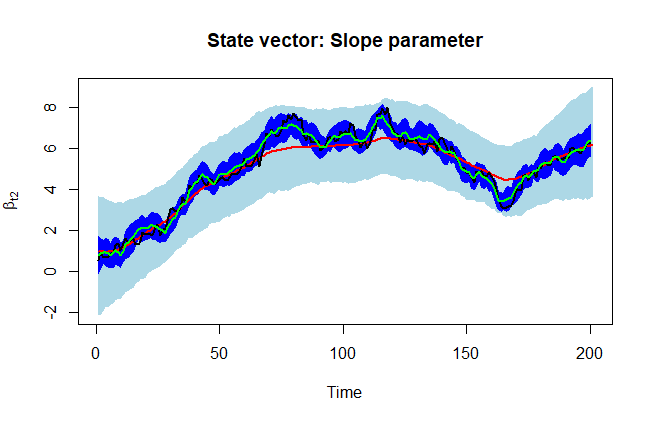
\includegraphics[width=340pt, height=200pt]{Chapters/chapter8/figures/SimSSreg.png}
	\caption[List of figure caption goes here]{Simulation: Dynamic linear model.}\label{fig1}
\end{figure} 

\textbf{Example: Effects of inflation on interest rate I}

We use the dataset \textit{16INTDEF.csv} provided by \cite[Chaps.~10]{wooldridge2016introductory} to study the effects of inflation on interest rate. The specification is $\Delta i_t=\beta_{t1}+\beta_{t2}\Delta inf_t+\beta_{t3}\Delta def_t+\mu_t$ and $\bm{\beta}_t=\bm{\beta}_{t-1}+\bm{w}_t$, where $\Delta z_t=z_{t}-z_{t-1}$ is the difference operator, $i_t$ is the three-month T-bill rate, $inf_t$ is the annual inflation rate based on the consumer price index (CPI), and $def_t$ is the federal budget deficit as percentage of gross domestic product (GDP) from 1948 to 2003 in the USA. In addition, $\mu_t\sim N(0,\sigma^2)$, $\bm{w}_t\sim N(\bm{0},\text{diag}\left\{\omega_1^2,\omega_1^2\right\})$. We assume inverse-gamma distributions for the priors of scale parameters, and set 12000 MCMC iterations, 2000 as burn-in, and 10 the thinning parameter.

The following code shows how to perform this application. We use the variance of the recursive estimation of the OLS to set the hyperparameters of the inverse-gamma distribution for the variance of $\bm{w}_t$, and the OLS estimate of the variance of the model to set the hyperparameters of the distribution of $\sigma^2$.

Figure \ref{fig2} shows the posterior results of the effect of the inflation on the interest rate. This is a fan chart indicating deciles from 10\% to 90\%, the red shadow area shows around the median value, and the black line is the mean value of the state associated with the annual change in inflation. We see that the annual changes in interest rate are weakly positive related to annual changes in inflation. 

\begin{tcolorbox}[enhanced,width=4.67in,center upper,
	fontupper=\large\bfseries,drop shadow southwest,sharp corners]
	\textit{R code. Dynamic linear model: Effects of inflation on interest rate}
	\begin{VF}
		\begin{lstlisting}[language=R]
rm(list = ls()); set.seed(010101)
DataIntRate <- read.csv("https://raw.githubusercontent.com/besmarter/BSTApp/refs/heads/master/DataApp/16INTDEF.csv", sep = ",", header = TRUE, quote = "")
attach(DataIntRate); Xt <- cbind(diff(inf), diff(def))
K <- dim(Xt)[2] + 1; yt <- diff(i3)
T <- length(yt); RegLS <- lm(yt ~ Xt)
SumRegLS <- summary(RegLS); SumRegLS; SumRegLS$sigma^2  
# Recursive OLS
Bp <- matrix(RegLS$coefficients, T, K, byrow = TRUE)
S <- 20
for(t in S:T){
	RegLSt <- lm(yt[1:t] ~ Xt[1:t,])
	Bp[t,] <- RegLSt$coefficients 
}
VarBp <- var(Bp)
# State spece model
ModelReg <- function(par){
	Mod <- dlm::dlmModReg(Xt, dV = exp(par[1]), dW = exp(par[2:(K+1)]), m0 = RegLS$coefficients,
	C0 = diag(VarBp))
	return(Mod)
}
MCMC <- 12000; burnin <- 2000; thin <- 10
gibbsOut <- dlm::dlmGibbsDIG(yt, mod = dlm::dlmModReg(Xt), a.y = 0.1, rate.y = 0.1,
shape.theta = 0.1, rate.theta = 0.1,
n.sample = MCMC,
thin = thin, save.states = TRUE)
B2t <- matrix(0, MCMC - burnin, T + 1)
for(t in 1:(T+1)){
	B2t[,t] <- gibbsOut[["theta"]][t,2,-c(1:burnin)] 
}
dV <- coda::mcmc(gibbsOut[["dV"]][-c(1:burnin)])
dW <- coda::mcmc(gibbsOut[["dW"]][-c(1:burnin),])
summary(dV); summary(dW)
plot(dV); plot(dW)
library(fanplot)
df <- as.data.frame(B2t)
plot(NULL, main="Percentiles", xlim = c(1, T+1), ylim = c(-1, 2), xlab = "Time", ylab = TeX("$\\beta_{t1}$"))
fan(data = df); lines(colMeans(B2t), col = "black", lw = 2)
abline(h=0, col = "blue")
\end{lstlisting}
	\end{VF}
\end{tcolorbox}

\begin{figure}[!h]
	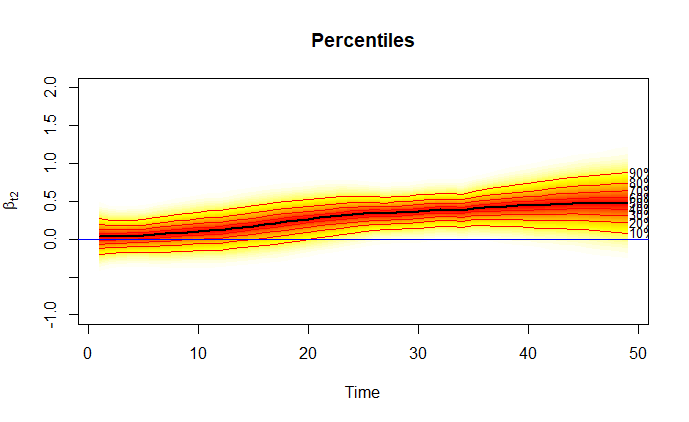
\includegraphics[width=340pt, height=200pt]{Chapters/chapter8/figures/IntInf.png}
	\caption[List of figure caption goes here]{Effects of inflation on interest rate: Dynamic linear model.}\label{fig2}
\end{figure}


We can extend the \textit{dynamic linear model} with \textit{random walk states} to take into account time invariant location parameters. In particular, we follow \cite{de1995simulation}, who propose the \textit{simulation smoother}. This algorithm overcomes some shortcomings of the FFBS algorithm, such as slow convergence and computational overhead. We focus on the case $M=1$, 
\begin{align}
	{Y}_t&=\bm{z}_t^{\top}\bm{\alpha}+\bm{x}_t^{\top}\bm{\beta}_t+\bm{h}_t^{\top}\bm{\epsilon}_t,& t=1,2,\dots,T. & \text{   (Observation equation)}\label{DeJongObs}\\
	\bm{\beta}_t&=\bm{\beta}_{t-1}+\bm{H}_t\bm{\epsilon}_t, & t=1,2,\dots,T. & \text{   (States equations)}\label{DeJongSt},
\end{align}
where $\bm{z}_t$ and $\bm{x}_t$ are $L$-dimensional and $K$-dimensional vectors of regressors associated with time-invariant and time-varying parameters, respectively, $\bm{h}_t$ is a vector of dimension $1+K$, $\bm{H}_t$ is a matrix of dimension $K\times 1+K$, $\bm{\beta}_0=\bm{0}$ and $\bm{\epsilon}_t\sim N(\bm{0}_{1+K},\sigma^2\bm{I}_{1+K})$.

Observe that this specification encompasses Equations \ref{eq1Obs} and \ref{eq1St} setting $\bm{\epsilon}_t=[\mu_t \ \bm{w}_t^{\top}]^{\top}$, $\bm{h}_t=[1 \ 0 \ \dots \ 0]$, $\bm{H}_t=[\bm{0}_K \ \bm{U}_{K\times K}]$ such that $\text{diag}\left\{\omega_1^2 \ \dots \ \omega_K^2\right\}=\sigma^2\bm{U}\bm{U}^{\top}$, $\bm{\alpha}=\bm{0}$, and $\bm{h}_t\bm{H}_t^{\top}=\bm{0}_{K}$.

The nice idea of \cite{de1995simulation} was to propose an efficient algorithm to get draws from $\bm{\eta}_t=\bm{F}_t\bm{\epsilon}_t$, where the most common choice is $\bm{F}_t=\bm{H}_t$, which means drawing samples from the perturbations of the states, and then, recovering the states from Equation \ref{DeJongSt} and $\bm{\beta}_0=\bm{0}$. \cite{de1995simulation} present a more general version of the \textit{state space model} that the one presented here. 

Using the system given by Equations \ref{DeJongObs} and \ref{DeJongSt}, $\bm{F}_t=\bm{H}_t$ and $\bm{h}_t\bm{H}_t^{\top}=\bm{0}_{K}$, the \textit{filtering} recursions are given by $e_t=Y_t-\bm{z}_t^{\top}\bm{\alpha}-\bm{x}_t^{\top}\bm{b}_{t-1}$, ${q}_t=\bm{x}_t^{\top}\bm{B}_{t-1}\bm{x}_t+\bm{h}_t^{\top}\bm{h}_t$, $\bm{K}_t=\bm{B}_{t-1}\bm{x}_tq_t^{-1}$, $\bm{b}_t=\bm{b}_{t-1}+\bm{K}_t e_t$, and $\bm{B}_t=\bm{B}_{t-1}-\bm{B}_{t-1}\bm{x}_t\bm{K}_t^{\top}+\bm{H}_t\bm{H}_t^{\top}$, where $\bm{b}_0=\bm{0}$ and $\bm{B}_0=\bm{H}_0\bm{H}_0^{\top}$. See system 2 in \cite{de1995simulation} for a more general case. We should save $e_t$ (innovation vector), $q_t$ (scale innovation variance) and $\bm{K}_t$ (\textit{Kalman gain}) from this recursion. 

Then, setting $\bm{r}_T=0$ and $\bm{M}_T=\bm{0}$, we run backwards from $t=T-1, T-2, \dots, 1$, the following recursions: $\bm{\Lambda}_{t+1}=\bm{H}_{t+1}\bm{H}_{t+1}^{\top}$, $\bm{C}_{t+1}=\bm{\Lambda}_{t+1}-\bm{\Lambda}_{t+1}\bm{M}_{t+1}\bm{\Lambda}_{t+1}^{\top}$, $\bm{\xi}_{t+1}\sim N(\bm{0}_K,\sigma^2\bm{C}_{t+1})$, $\bm{L}_{t+1}=\bm{I}_K-\bm{K}_{t+1}\bm{x}_{t+1}^{\top}$, $\bm{V}_{t+1}=\bm{\Lambda}_{t+1}\bm{M}_{t+1}\bm{L}_{t+1}$, $\bm{r}_{t}=\bm{x}_{t+1} e_{t+1}/q_{t+1} + \bm{L}_{t+1}^{\top}\bm{r}_{t+1}-\bm{V}_{t+1}^{\top}\bm{C}_{t+1}^{-1}\bm{\xi}_{t+1}$, $\bm{M}_{t}=\bm{x}_{t+1}\bm{x}_{t+1}^{\top}/q_{t+1}+\bm{L}_{t+1}^{\top}\bm{M}_{t+1}\bm{L}_{t+1}+\bm{V}_{t+1}^{\top}\bm{C}_{t+1}^{-1}\bm{V}_{t+1}$, and $\bm{\eta}_{t+1}=\bm{\Lambda}_{t+1}\bm{r}_{t+1}+\bm{\xi}_{t+1}$. \cite{de1995simulation} show that $\bm{\eta}=[\bm{\eta}_1^{\top} \ \dots \ \bm{\eta}_T^{\top}]^{\top}$ is drawn from $p(\bm{H}_t\bm{\epsilon}_t|y_t,\bm{x}_t,\bm{z}_t,\bm{h}_t,\bm{H}_t,\bm{\alpha},\sigma^2, t=1,2,\dots,T)$. Thus, we can recover $\bm{\beta}_t$ using \ref{DeJongSt} and $\bm{\beta}_0=\bm{0}_K$.

We assume in the model given by Equations \ref{DeJongObs} and \ref{DeJongSt} that $\bm{h}_t=[1 \ 0 \ \dots \ 0]^{
\top}$ and $\bm{H}_t=[\bm{0}_K \ \text{diag}\left\{1/\tau_1\dots1/\tau_K\right\}]$, and then perform Bayesian inference assuming independent priors, that is, $\pi(\bm{\beta}_0,\bm{\alpha},\sigma^2,\bm{\tau})=\pi(\bm{\beta}_0)\pi(\bm{\alpha})\pi(\sigma^2)\prod_{k=1}^K\pi(\tau_k^2)$ where $\sigma^2\sim IG(\alpha_0/2,\delta_0/2)$, $\tau_k^2\sim G(v_{0}/2,v_{0}/2)$, $k=1,\dots,K$, $\bm{\alpha}\sim N(\bm{a}_0,\bm{A}_0)$ and $\bm{\beta}_0\sim N(\bm{b}_0,\bm{B}_0)$. The conditional posterior distributions are $\sigma^2|\bm{y},\bm{X},\bm{Z},\bm{\beta}_{0:T},\bm{\alpha},\bm{\tau}\sim IG(\alpha_{n}/2,\delta_n/2)$, where $\delta_n=\sum_{t=1}^T\left[(\bm{\beta}_t-\bm{\beta}_{t-1})^{\top}\bm{\Psi}(\bm{\beta}_t-\bm{\beta}_{t-1})+(y_t-\bm{z}_t^{\top}\bm{\alpha}-\bm{x}_t^{\top}\bm{\beta}_t)^{\top}(y_t-\bm{z}_t^{\top}\bm{\alpha}-\bm{x}_t^{\top}\bm{\beta}_t)\right]+\delta_0$ and  $\alpha_{n}=T(K+1)+\alpha_0$, $\bm{\tau}=[\tau_1 \ \dots \ \tau_K]$, $\bm{\Psi}=\text{diag}\left\{\tau_1^2,\dots,\tau_K^2\right\}$, and $\tau_k^2|\bm{y},\bm{X},\bm{Z},\bm{\beta}_{0:T},\sigma^2\sim G(v_{1n}/2,v_{2kn}/2)$, where $v_{1n}=T+v_{0}$ and $v_{2kn}=\sigma^{-2}\sum_{t=1}^T(\bm{\beta}_{t,k}-\bm{\beta}_{t-1,k})^2+v_{0}$, and $\bm{\alpha}|\bm{y},\bm{X},\bm{Z},\sigma^2,\bm{\beta}_{1:T},\bm{\tau}\sim N(\bm{a}_n,\bm{A}_n)$, where $\bm{A}_n=(\bm{A}_0^{-1}+\sigma^{-2}\sum_{t=1}^T\bm{z}_t\bm{z}_t^{\top})^{-1}$ and $\bm{a}_n=\bm{A}_n(\bm{A}_0^{-1}\bm{a}_0+\sigma^{-2}\sum_{t=1}^T\bm{z}_t(y_t-\bm{x}_t^{\top}\bm{\beta}_t))$. The vector of the dependent variable is $\bm{y}$, and all regressors are in $\bm{X}$ and $\bm{Z}$.

We can see that all the previous posterior distributions are conditional on the state vector $\bm{\beta}_{0:T}$, which can be sampled using the \textit{simulation smoother} algorithm conditional on draws of the time-invariant parameters. Thus, the \textit{state space model} provides an excellent illustration of the modular nature of the Bayesian framework where performing inference of more complex models very often simply involves adding new blocks to a MCMC algorithm. This means we can break down a complex inferential problem into smaller, more manageable parts, this is, a ``divide and conquer" approach. This is possible due to the structure of conditional posterior distributions. Exercise 3 asks to perform a simulation of the model given by Equations \ref{DeJongObs} and \ref{DeJongSt}, and program the MCMC algorithm including the \textit{simulation smoother}.   

\section{ARMA processes}\label{sec82}

Since the seminal work of \cite{box_jenkins_1976}, autoregressive moving average (ARMA) models have become ubiquitous in time series analysis. Thus, we present a brief introduction to these models in this section.

Let's start with the linear Gaussian model with autorregresive errors,
\begin{align}
	Y_t & = \bm{x}_t^{\top}\bm{\beta}+\mu_t\label{eq1}\\
	\phi(L)\mu_t & = \epsilon_t \label{eq2}, 
\end{align}
where $\epsilon_t \stackrel{iid}{\sim} N(0,\sigma^2)$, $\phi(L)=1-\phi_1L-\phi_2L^2-\dots-\phi_pL^p$ is a polynomial in the lag operator ($L$), where $Lz_t=z_{t-1}$, and in general, $L^rz_t=z_{t-r}$.

Thus, we see that stochastic error $\mu_t$ follows an \textit{autoregressive process of order $p$}, that is, $\mu_t\sim AR(p)$. It is standard practice to assume that $\mu_t$ is second-order stationary, this implies that the mean, variance and autocovariance of $\mu_t$ are finite and independent of $t$ and $s$, although $\mathbb{E}[\mu_t\mu_s]$ may depend on $|t-s|$. Then, all roots of $\phi(L)$ lie outside the unit circle, for instance, given an $AR(1)$, then, $1-\phi_1L=0$, implies, $L=1/\phi_1$ such that  $|\phi_1|<0$ for the process being second-order stationary.

The likelihood function conditional on the first $p$ observations is
\begin{align*}
	p(Y_{p+1},\dots,Y_T|y_{p},\dots,y_1,\bm{\theta})&=\prod_{t=p+1}^{T}p(Y_t|H_{t-1},\bm{\theta})\\
	&\propto \sigma^{-(T-p)}\exp\left\{-\frac{1}{2\sigma^2}\sum_{t=p+1}^T(Y_t-\hat{Y}_{t|t-1,\bm{\theta}})^2\right\},
\end{align*} 
where $H_{t-1}$ is the past history, $\bm{\theta}$ collects all parameters ($\bm{\beta}, \phi_1,\dots,\phi_p, \sigma^2$), and $\hat{Y}_{t|t-1,\bm{\theta}}=(1-\phi(L))Y_t+\phi(L)\bm{x}^{\top}\bm{\beta}$.

We can see that multiplying the first expression in Equation \ref{eq1} by $\phi(L)$, we can express the model as 
\begin{align}\label{eq3}
	Y_t^*=\bm{x}_t^{*\top}\bm{\beta}+\epsilon_t
\end{align}
where $Y_t^*=\phi(L)Y_t$ and $\bm{x}_t^{*}=\phi(L)\bm{x}_t$.

Thus, collecting all observations $t=p+1,p+2,\dots,T$, we have $\bm{y}^*=\bm{X}^*\bm{\beta}+\bm{\epsilon}$, where $\bm{\epsilon}\sim N(\bm{0},\sigma^2\bm{I}_{T-p})$, $\bm{y}^*$ is a $T-p$ dimensional vector, and $\bm{X}^*$ is a $(T-p)\times K$ dimensional matrix.

Assuming that $\bm{\beta}|\sigma\sim N(\bm{\beta}_0,\sigma^2\bm{B}_0)$, $\sigma^2\sim IG(\alpha_0/2,\delta_0/2)$ and $\bm{\phi}\sim N(\bm{\phi}_0,\bm{\Phi}_0)\mathbbm{1}[\bm{\phi}\in S_{\bm{\phi}}]$, where $S_{\bm{\phi}}$ is the stationary region of $\bm{\phi}=[\phi_1 \ \dots \ \phi_p]^{\top}$. Then, Equation \ref{eq3} implies that $\bm{\beta}|\sigma^2,\bm{\phi},\bm{y},\bm{X}\sim N(\bm{\beta}_n, \sigma^2{\bf{B}}_n)$, where $\bm{B}_n = (\bm{B}_0^{-1} + \bm{X}^{*\top}\bm{X}^{*})^{-1}$ and $\bm{\beta}_n = \bm{B}_n(\bm{B}_0^{-1}\bm{\beta}_0 + \bm{X}^{*\top}\bm{y}^{*})$. In addition, $\sigma^2|\bm{\beta},\bm{\phi},\bm{y},\bm{X}\sim IG(\alpha_n/2,\delta_n/2)$ where $\alpha_n=\alpha_0+T-p$ and $\delta_n=\delta_0+(\bm{y}^*-\bm{X}^{*}\bm{\beta})^{\top}(\bm{y}^*-\bm{X}^{*}\bm{\beta})+(\bm{\beta}-\bm{\beta}_0)\bm{B}_0^{-1}(\bm{\beta}-\bm{\beta}_0)$. Thus, the previous conditional posterior distributions imply that we can use a Gibbs sampling algorithm to perform inference of these parameters \cite{chib1993bayes}.

We know from Equation \ref{eq1} that $\mu_t=Y_t-\bm{x}_t^{\top}\bm{\beta}$, from Equation \ref{eq2} that $\mu_t=\phi_1\mu_{t-1}+\dots+\phi_p\mu_{t-p}+\epsilon_t$, $t=p+1,\dots,T$. In matrix notation $\bm{\mu}=\bm{U}\bm{\phi}+\bm{\epsilon}$, where $\bm{\mu}$ is a $T-p$ dimensional vector, $\bm{U}$ is a $(T-p)\times p$ matrix whose $t$-th row is $[\mu_{t-1} \ \dots \ \mu_{t-p}]$. Thus, the posterior distribution of $\bm{\phi}|\bm{\beta},\sigma^2,\bm{y},\bm{X}$ is $N(\bm{\phi}_n, \bm{\Phi}_n)\mathbbm{1}[\bm{\phi}\in S_{\bm{\phi}}]$, where $\bm{\Phi}_n=(\bm{\Phi}_0^{-1}+\sigma^{-2}\bm{U}^{\top}\bm{U})$ and $\bm{\phi}_n=\bm{\Phi}_n(\bm{\Phi}_0^{-1}\bm{\phi}_0+\sigma^{-2}\bm{U}^{\top}\bm{\mu})$ (see Exercise 4).

Drawing from the model restricted to stationarity is straightforward: we simply sample from the multivariate normal distribution and discard draws that do not meet the stationarity condition. The proportion of draws that satisfy this restriction represents the conditional probability that the process is stationary.\\

\textbf{Example: Effects of inflation on interest rate II}

We specified a \textit{dynamic linear model} in the example of the effects of inflation on interest rate to take into account a potential dynamic relationship. However, we can consider dynamics in this example assuming  $\Delta i_t=\beta_{1}+\beta_{2}\Delta inf_t+\beta_{3}\Delta def_t+\mu_t$ where $\mu_t=\phi \mu_{t-1} + \epsilon_t$, which implies $\Delta i_t=\beta_{1}(1-\phi_1)+\phi_1\Delta i_{t-1}+\beta_{2}(\Delta inf_t-\phi_1 \Delta inf_{t-1})+\beta_{3}(\Delta def_t-\phi_1 \Delta def_{t-1})+\epsilon_t$. Thus, we use again the dataset \textit{16INTDEF.csv} provided by \cite[Chaps.~10]{wooldridge2016introductory} to provide an illustration of linear regressions with $AR(1)$ errors.

The following code shows how to perform this application using vague priors assuming $\alpha_0=\delta_0=0.01$, $\bm{\beta}_0=\bm{0}$, $\bm{B}_0=\bm{I}$, $\bm{\phi}_0=\bm{0}$ and $\bm{\Phi}_0=\bm{I}$. We use 15000 MCMC iterations plus a burn-in equal 5000, and thin equal to 5. 


\begin{tcolorbox}[enhanced,width=4.67in,center upper,
	fontupper=\large\bfseries,drop shadow southwest,sharp corners]
	\textit{R code. AR(1) model: Effects of inflation on interest rate}
	\begin{VF}
		\begin{lstlisting}[language=R]
rm(list = ls())
set.seed(010101)
DataIntRate <- read.csv("https://raw.githubusercontent.com/besmarter/BSTApp/refs/heads/master/DataApp/16INTDEF.csv", sep = ",", header = TRUE, quote = "")
attach(DataIntRate)
yt <- diff(i3); ytlag <- dplyr::lag(yt, n = 1)
T <- length(yt)
Xt <- cbind(diff(inf), diff(def)); Xtlag <- dplyr::lag(Xt, n = 1)
K <- dim(Xt)[2] + 1
Reg <- lm(yt ~ ytlag + I(Xt[,-1] - Xtlag))
SumReg <- summary(Reg); SumReg
PostSig2 <- function(Beta, Phi){
	Xstar<- matrix(NA, T-1, K - 1)
	ystar <- matrix(NA, T-1, 1)
	for(t in 2:T){
		Xstar[t-1,] <- Xt[t,] - Phi*Xt[t-1,]
		ystar[t-1,] <- yt[t] - Phi*yt[t-1]
	}
	Xstar <- cbind(1, Xstar)
	an <- T - 1 + a0
	dn <- d0 + t(ystar - Xstar%*%Beta)%*%(ystar - Xstar%*%Beta) + t(Beta - b0)%*%B0i%*%(Beta - b0)
	sig2 <- invgamma::rinvgamma(1, shape = an/2, rate = dn/2)
	return(sig2)
}
PostBeta <- function(sig2, Phi){
	Xstar<- matrix(NA, T-1, K - 1)
	ystar <- matrix(NA, T-1, 1)
	for(t in 2:T){
		Xstar[t-1,] <- Xt[t,] - Phi*Xt[t-1,]
		ystar[t-1,] <- yt[t] - Phi*yt[t-1]
	}
	Xstar <- cbind(1, Xstar)
	XtXstar <- t(Xstar)%*%Xstar
	Xtystar <- t(Xstar)%*%ystar
	Bn <- solve(B0i + XtXstar)
	bn <- Bn%*%(B0i%*%b0 + Xtystar)
	Beta <- MASS::mvrnorm(1, bn, sig2*Bn)
	return(Beta)
}
PostPhi <- function(sig2, Beta){
	u <- yt - cbind(1,Xt)%*%Beta
	U <- u[-T]
	ustar <- u[-1]
	UtU <- t(U)%*%U
	Utu <- t(U)%*%ustar
	Phin <- solve(Phi0i + sig2^(-1)*UtU)
	phin <- Phin%*%(Phi0i%*%phi0 + sig2^(-1)*Utu)
	Phi <- truncnorm::rtruncnorm(1, a = -1, b = 1, mean = phin, sd = Phin^0.5)
	return(Phi)
}
		\end{lstlisting}
	\end{VF}
\end{tcolorbox}


\begin{tcolorbox}[enhanced,width=4.67in,center upper,
	fontupper=\large\bfseries,drop shadow southwest,sharp corners]
	\textit{R code. AR(1) model: Effects of inflation on interest rate}
	\begin{VF}
		\begin{lstlisting}[language=R]
# Hyperparameters
d0 <- 0.01; a0 <- 0.01
b0 <- rep(0, K); c0 <- 1; 
B0 <- c0*diag(K); B0i <- solve(B0)
phi0 <- 0; Phi0 <- 1; Phi0i <- 1/Phi0
# MCMC parameters
mcmc <- 15000
burnin <- 5000
tot <- mcmc + burnin
thin <- 1
PostBetas <- matrix(0, mcmc+burnin, K)
PostSigma2s <- rep(0, mcmc+burnin)
PostPhis <- rep(0, mcmc+burnin)
Beta <- rep(0, K); Phi <- 0
sig2 <- SumReg$sigma^2; Phi <- SumReg$coefficients[2,1]
Beta <- SumReg$coefficients[c(1,3,4),1]
pb <- winProgressBar(title = "progress bar", min = 0, max = tot, width = 300)
for(s in 1:tot){
	sig2 <- PostSig2(Beta = Beta, Phi = Phi)
	PostSigma2s[s] <- sig2
	Beta <- PostBeta(sig2 = sig2, Phi = Phi)
	PostBetas[s,] <- Beta
	Phi <- PostPhi(sig2 = sig2, Beta = Beta)
	PostPhis[s] <- Phi
	setWinProgressBar(pb, s, title=paste( round(s/tot*100, 0), "% done"))
}
close(pb)
keep <- seq((burnin+1), tot, thin)
PosteriorBetas <- coda::mcmc(PostBetas[keep,])
summary(PosteriorBetas)
PosteriorSigma2 <- coda::mcmc(PostSigma2s[keep])
summary(PosteriorSigma2)
PosteriorPhi <- coda::mcmc(PostPhis[keep])
summary(PosteriorPhi)
dfBinf <- as.data.frame(PosteriorBetas[,2])
# Basic density
p <- ggplot(dfBinf, aes(x=var1)) + 
geom_density(color="darkblue", fill="lightblue") +
geom_vline(aes(xintercept=mean(var1)), color="blue", linetype="dashed", linewidth=1) +
geom_vline(aes(xintercept=quantile(var1, 0.025)), color="red", linetype="dashed", linewidth=1) +
geom_vline(aes(xintercept=quantile(var1, 0.975)), color="red", linetype="dashed", linewidth=1) +
labs(title="Density effect of inflation on interest rate", x="Effect of inflation", y = "Density")
\end{lstlisting}
	\end{VF}
\end{tcolorbox}

Figure \ref{fig3} shows the posterior density plot of the effects of inflation rate on interest rate. The posterior mean of this coefficient is approximately 0.25, and the credible interval at 95\% is (0, 0.46), which indicates again that the annual changes in interest rate are weakly positive related to annual changes in inflation (see Figure \ref{fig2} as reference). 

\begin{figure}[!h]
	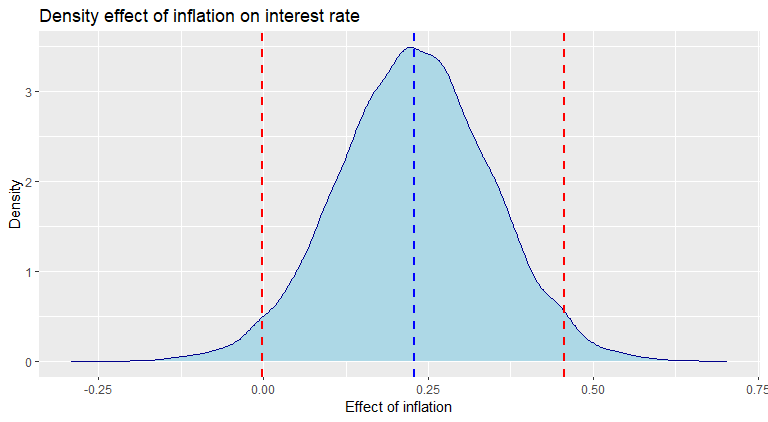
\includegraphics[width=340pt, height=200pt]{Chapters/chapter8/figures/InfInt.png}
	\caption[List of figure caption goes here]{Density: Effects of inflation on interest rate.}\label{fig3}
\end{figure} 


Observe that the previous setting encompasses the particular relevant case  $Y_t\sim AR(p)$, it is just omitting the covariates such that $Y_t=\mu_t$. \cite{chib1994bayes} extend the Bayesian inference of linear regression with $AR(p)$ errors to $ARMA(p,q)$ errors using a \textit{state-space} representation. 

Setting $Y_t=\mu_t$ such that $Y_t=\sum_{s=1}^{p}\phi_jY_{t-s}+\sum_{s=1}^{q}\theta_s \epsilon_{t-s}+\epsilon_t$, letting $r=\max \left\{p,q+1\right\}$, $\phi_s=0$ for $s>p$ and $\theta_s=0$ for $s>q$, and defining the matrices $\bm{x}^{\top}=[1 \ 0 \ \dots \ 0]$, $\bm{H}=[1 \ \psi_1 \ \dots \ \psi_{r-1}]^{\top}$, both are $r$-dimensional vectors, 
\begin{align*}
	\bm{G}=\begin{bmatrix}
		\phi_1 & 1 & 0 & \dots & 0\\
		\phi_2 & 0 & 1 & \dots & 0\\
		\vdots & \vdots & \ddots &  &\\
		\phi_{r-1} & 0 & 0 & \dots & 1\\
		\phi_r & 0 & 0 & \dots & 0\\
	\end{bmatrix} = \begin{bmatrix}
		\phi_1 & \vdots &  &  & \\
		\phi_2 & \vdots &  & \bm{I}_{r-1}  & \\
		\vdots & \vdots &  &  &\\
		\dots & \dots & \dots & \dots & \dots\\
		\phi_r & 0 & 0 & \dots & 0\\
	\end{bmatrix},
\end{align*} 
which is a $r\times r$ dimensional matrix, and give the \textit{state} vector $\bm{\beta}_t=[\beta_{1,t} \ \beta_{2,t} \ \dots \ \beta_{r,t}]^{\top}$, the $ARMA$ model has the following representation:
\begin{align*}
	Y_t&=\bm{x}^{\top}\bm{\beta}_t\\
	\bm{\beta}_t &= \bm{G}\bm{\beta}_{t-1}+\bm{H}\epsilon_{t}.
\end{align*}

This is a \textit{dynamic linear model} where $\bm{\Sigma}_t=0$, and $\bm{\Omega}_t=\sigma^2\bm{H}\bm{H}^{\top}$ (see \cite{petris2009dynamic,chib1994bayes}).

A nice advantage of the \textit{state-space} representation of the $ARMA$ model is that the evaluation of the likelihood can be performed efficiently using the recursive laws. Extensions to autoregressive integrated moving average $ARIMA(p,d,q)$ models can be seen in \cite[Chap.~3]{petris2009dynamic}. In $ARIMA(p,d,q)$ models, $d$ refers to the level of integration (difference) that is required to eliminate the stochastic trend in a time series (see \cite[Chap.~4]{enders_2014} for details).\\

\textbf{Example: $AR(2)$ process}

Let's see the \textit{state-space} representation of a stationary $AR(2)$ process with intercept, that is, $Y_t=\mu+\phi_1Y_{t-1}+\phi_2Y_{t-2}+\epsilon_t$, where $\epsilon_t\sim N(0,\sigma^2)$. Thus, $\mathbb{E}[Y_t]=\frac{\mu}{1-\phi_1-\phi_2}$, and variance $Var[Y_t]=\frac{\sigma^2(1-\phi_2)}{1-\phi_2-\phi_1^2-\phi_1^2\phi_2-\phi_2^2+\phi_2^3}$.

In addition, we can proof that setting $z_t=Y_t-\bar{\mu}$, we have $z_t=\phi_1z_{t-1}+\phi_2z_{t-2}+\epsilon_t$ where $\mathbb{E}[z_t]=0$, and these are equivalent representations (see Exercise 5). Then, setting  $\bm{x}^{\top}=[1 \ 0]$, $\bm{H}=[1 \ 0]^{\top}$, $\bm{G}=\begin{bmatrix}
	\phi_1 & 1\\
	\phi_2 & 0 \\
\end{bmatrix}$, $\bm{\beta}_t=[\beta_{t1} \ \beta_{t2}]^{\top}$, $\bm{\Sigma}_t=0$ and $\bm{\Omega}_t=\sigma^2$ we have
\begin{align*}
	z_t&=\bm{x}^{\top}\bm{\beta}_t& \text{(Observation equations)}\\
	\bm{\beta}_t&=\bm{G}\bm{\beta}_{t-1}+\bm{H}{\epsilon}_t & \text{(States equations)}.
\end{align*}

We use the function \textit{stan\_sarima} from the package \textit{bayesforecast} to perform Bayesian inference in $ARMA$ models in our GUI. The following code shows how to simulate an $AR(2)$ process, and perform Bayesian inference using this function.

\begin{tcolorbox}[enhanced,width=4.67in,center upper,
	fontupper=\large\bfseries,drop shadow southwest,sharp corners]
	\textit{R code. Simulation and inference: AR(2) model}
	\begin{VF}
		\begin{lstlisting}[language=R]
rm(list = ls()); set.seed(010101)
T <- 200; mu <- 0.5 
phi1 <- 0.5; phi2 <- 0.3; sig <- 0.5
Ey <- mu/(1-phi1-phi2); Sigy <- sig*((1-phi2)/(1-phi2-phi1^2-phi2*phi1^2-phi2^2+phi2^3))^0.5 
y <- rnorm(T, mean = Ey, sd = Sigy)
e <- rnorm(T, mean = 0, sd = sig)
for(t in 3:T){
	y[t] <- mu + phi1*y[t-1] + phi2*y[t-2] + e[t]
}
mean(y); sd(y)
y <- ts(y, start=c(1820, 1), frequency=1)
plot(y)
iter <- 10000; burnin <- 5000; thin <- 1; tot <- iter + burnin
library(bayesforecast)
sf1 <- bayesforecast::stan_sarima(y, order = c(2, 0, 0), prior_mu0 = normal(0, 1),
prior_ar = normal(0, 1), prior_sigma0 = inverse.gamma(0.01/2, 0.01/2),
seasonal = c(0, 0, 0), iter = tot, warmup = burnin, chains = 1)
keep <- seq(burnin+1, tot, thin)
Postmu <- sf1[["stanfit"]]@sim[["samples"]][[1]][["mu0"]][keep]
Postsig <- sf1[["stanfit"]]@sim[["samples"]][[1]][["sigma0"]][keep]
Postphi1 <- sf1[["stanfit"]]@sim[["samples"]][[1]][["ar0[1]"]][keep]
Postphi2 <- sf1[["stanfit"]]@sim[["samples"]][[1]][["ar0[2]"]][keep]
Postdraws <- coda::mcmc(cbind(Postmu, Postsig, Postphi1, Postphi2))
summary(Postdraws)
Quantiles for each variable:
            	2.5%    25%    50%    75%  97.5%
Postmu   0.39914 0.5732 0.6625 0.7518 0.9346
Postsig  0.47696 0.5071 0.5248 0.5439 0.5829
Postphi1 0.42384 0.5159 0.5634 0.6089 0.6979
Postphi2 0.06034 0.1456 0.1920 0.2361 0.3286
plot(Postdraws)
\end{lstlisting}
	\end{VF}
\end{tcolorbox}
We perform 10000 MCMC iterations plus a burn-in equal 5000 assuming $\sigma^2\sim IG(0.01/2, 0.01/2)$, $\mu\sim N(0, 1)$ and $\phi_k\sim N(0, 1)$, $k=1,2$. The trace plots look well, and all 95\% credible intervals encompass the population values.

Algorithm \ref{alg:ARMA} shows how to do perform inference in $ARMA(p,q)$ models using our GUI. See also Chapter \ref{chapGUI} for details regarding the dataset structure. 

\begin{algorithm}[h!]
	\caption{Autoregressive Moving Average ($ARMA$) models}\label{alg:ARMA}
	\begin{algorithmic}[1]  		 			
		\State Select \textit{Time series Model} on the top panel
		\State Select \textit{ARMA} using the left radio button
		\State Upload the dataset selecting first if there is header in the file, and the kind of separator in the \textit{csv} file of the dataset (comma, semicolon, or tab). Then, use the \textit{Browse} button under the \textbf{Choose File} legend
		\State Select MCMC iterations, burn-in and thinning parameters using the \textit{Range sliders}
		\State Set the order of the $ARMA$ model, $p$ and $q$ parameters
		\State Set the location and scale hyperparameters of the \textit{intercept}, autoregressive ($AR$), moving average ($MA$) and standard deviation. This step is not necessary as by default our GUI uses non-informative priors
		\State Click the \textit{Go!} button
		\State Analyze results
		\State Download posterior chains and diagnostic plots using the \textit{Download Posterior Chains} and \textit{Download Posterior Graphs} buttons
	\end{algorithmic} 
\end{algorithm}

The function \textit{stan\_sarima} uses software \textit{Stan} \cite{Stan2024}, which in turn uses \textit{Hamiltonian Monte Carlo} (HMC) via no-U-turn sampler (NUTS) in the burn-in period. The following code shows how to perform Bayesian inference in the $AR(2)$ model programming the HMC from scratch. We should clarify that this is only an illustration, as HMC is less efficient than the Gibbs sampler in this example. However, HMC can outperform traditional MCMC algorithms in more complex models, especially when dealing with high-dimensional probability distributions or when MCMC struggles with poor mixing due to posterior correlation.

We perform the simulation in the first block, and then set the hyperparameters, and the function to calculate the logarithm of the posterior distribution. We parametrize the model using $\tau = \log(\sigma^2)$ such that $\sigma^2=\exp\left\{\tau\right\}$, consequently, avoiding issues due to the restriction of non-negativity of $\sigma^2$. Thus, we must take into account the Jacobian due to the transformation, that is $d\sigma^2/d\tau=\exp(\tau)$. Then, we have the function to calculate the gradient vector of the log posterior distribution. We should calculate the gradient vector analytically because using finite difference can be computationally expensive. However, it can be a good idea to check the analytical calculations evaluation the function at the maximum posterior estimate, where this function should return values near 0.

The posterior distribution is given by\footnote{Take into account that we do not consider the first two observations when present the likelihood, this is no an issue when there is a large sample size.}
\begin{align*}
	\pi(\mu,\phi_1,\phi_2,\tau|\bm{y})&\propto \prod_{t=3}^T(\exp(\tau))^{-1/2}\exp\left\{-\frac{1}{2\exp(\tau)}(y_t-\mu-\phi_1y_{t-1}-\phi_2y_{t-2})^2\right\}\\
	&\times\exp\left\{-\frac{1}{2\sigma^2_{\mu}}(\mu-\mu_0)^2\right\}\times\exp\left\{-\frac{1}{2\sigma^2_{\phi_1}}(\phi_1-\phi_{10})^2\right\}\\
	&\times\exp\left\{-\frac{1}{2\sigma^2_{\phi_2}}(\phi_2-\phi_{20})^2\right\}\times\exp\left\{-(\alpha_0/2+1)\tau\right\}\exp\left\{-\delta_0/(2\exp(\tau))\right\}\exp(\tau).
\end{align*} 

The components of the gradient vector of the log posterior distribution are given by
\begin{align*}
	\frac{\partial \log(\pi(\mu,\phi_1,\phi_2,\tau|\bm{y}))}{\partial\mu}&=\frac{\sum_{t=3}^T(y_t-\mu-\phi_1y_{t-1}-\phi_2y_{t-2})}{\exp(\tau)}-\frac{1}{\sigma_{\mu}^2}(\mu-\mu_0)\\
	\frac{\partial\log(\pi(\mu,\phi_1,\phi_2,\tau|\bm{y}))}{\partial\phi_1}&=\frac{\sum_{t=3}^T(y_t-\mu-\phi_1y_{t-1}-\phi_2y_{t-2})y_{t-1}}{\exp(\tau)}-\frac{1}{\sigma_{\phi_1}^2}(\phi_1-\phi_{10})\\
	\frac{\partial\log(\pi(\mu,\phi_1,\phi_2,\tau|\bm{y}))}{\partial\phi_2}&=\frac{\sum_{t=3}^T(y_t-\mu-\phi_1y_{t-1}-\phi_2y_{t-2})y_{t-2}}{\exp(\tau)}-\frac{1}{\sigma_{\phi_2}^2}(\phi_2-\phi_{20})\\	\frac{\partial\log(\pi(\mu,\phi_1,\phi_2,\tau|\bm{y}))}{\partial\tau}&=-\frac{(T-2)}{2}+\frac{\sum_{t=3}^T(y_t-\mu-\phi_1y_{t-1}-\phi_2y_{t-2})^2}{2\exp(\tau)}\\
	&-(\alpha_0/2+1)+\delta_0/(2\exp(\tau))+1.\\
\end{align*}

Then, we have the code for the Hamiltonian Monte Carlo as given in Chapter \ref{chap5}. We set the initial values equal to $\mu=\bar{y}=1/(T-2)\sum_{t=3}^T y_t$, $\phi_1=\phi_2=0$ and $\exp((1/(T-2))\sum_{t=3}^T(y_t-\bar{y})^2)$, and $M$ equal to the inverse covariance matrix of the posterior distribution evaluated at the maximum a posterior estimate. In addition, $\epsilon$ is randomly draw from a uniform distribution between 0 and 2$\epsilon_0$, and $L$ is the highest integer near to $1/\epsilon$, this to approximately satisfy $L\epsilon=1$. 

We can check that all 95\% credible intervals encompass the population values, and the posterior means are near the population values. The acceptance rate is higher than 65\% on average, thus we should increase the base step ($\epsilon_0$) from 0.1 to 0.2. In addition, we do not impose the stationary conditions on $\phi_1$ and $\phi_2$. Exercise 6 asks to program a HMC taking into account these requirements.

\begin{tcolorbox}[enhanced,width=4.67in,center upper,
	fontupper=\large\bfseries,drop shadow southwest,sharp corners]
	\textit{R code. Simulation and inference: AR(2) model using Hamiltonian Monte Carlo}
	\begin{VF}
		\begin{lstlisting}[language=R]
# Simulation AR(2)
rm(list = ls()); set.seed(010101); T <- 1000; K <- 4 
mu <- 0.5; phi1 <- 0.5; phi2 <- 0.3; sig <- 0.5 
Ey <- mu/(1-phi1-phi2); Sigy <- sig*((1-phi2)/(1-phi2-phi1^2-phi2*phi1^2-phi2^2+phi2^3))^0.5 
y <- rnorm(T, mean = Ey, sd = Sigy); e <- rnorm(T, mean = 0, sd = sig)
for(t in 3:T){
	y[t] <- mu + phi1*y[t-1] + phi2*y[t-2] + e[t]
}
# Hyperparameters
d0 <- 0.01; a0 <- 0.01; mu0 <- 0; MU0 <- 1
phi0 <- c(0, 0); Phi0 <- diag(2)
# Log posterior multiply by -1 to use optim
LogPost <- function(theta, y){
	mu <- theta[1]; phi1 <- theta[2]; phi2 <- theta[3]
	tau <- theta[4]; sig2 <- exp(tau); logLik <- NULL
	for(t in 3:T){
		logLikt <- dnorm(y[t], mean = mu + phi1*y[t-1] + phi2*y[t-2], sd = sig2^0.5, log = TRUE)
		logLik <- c(logLik, logLikt)
	}
	logLik <- sum(logLik)
	logPrior <- dnorm(mu, mean = mu0, sd = MU0^0.5, log = TRUE) + dnorm(phi1, mean = phi0[1], sd = Phi0[1,1]^0.5, log = TRUE) + dnorm(phi2, mean = phi0[2], sd = Phi0[2,2]^0.5, log = TRUE) + invgamma::dinvgamma(sig2, shape = a0/2, rate = d0/2, log = TRUE)
	logPosterior <- logLik + logPrior + tau
	return(-logPosterior) # Multiply by -1 to minimize using optim
}
theta0 <- c(mean(y), 0, 0, var(y))
Opt <- optim(theta0, LogPost, y = y, hessian = TRUE)
theta0 <- Opt$par; VarPost <- solve(Opt$hessian)
# Gradient log posterior
GradientTheta <- function(theta, y){
	mu <- theta[1]; phi1 <- theta[2]; phi2 <- theta[3]
	tau <- theta[4]; sig2 <- exp(tau); SumLik <- matrix(0, 3, 1)
	SumLik2 <- NULL
	for(t in 3:T){
		xt <- matrix(c(1, y[t-1], y[t-2]), 3, 1)
		SumLikt <- (y[t] - (mu + phi1*y[t-1] + phi2*y[t-2]))*xt
		SumLik2t <- (y[t] - (mu + phi1*y[t-1] + phi2*y[t-2]))^2
		SumLik <- rowSums(cbind(SumLik, SumLikt))
		SumLik2 <- sum(SumLik2, SumLik2t)
	}
	Grad_mu <- SumLik[1]/sig2 - (1/MU0)*(mu - mu0)
	Grad_phi1 <- SumLik[2]/exp(tau) - 1/Phi0[1,1]*(phi1 - phi0[1])
	Grad_phi2 <- SumLik[3]/exp(tau) - 1/Phi0[2,2]*(phi2 - phi0[2])
	Grad_tau <- -(T-2)/2 + SumLik2/(2*exp(tau)) - (a0/2 + 1) + d0/(2*exp(tau)) + 1 
	Grad <- c(Grad_mu, Grad_phi1, Grad_phi2, Grad_tau)
	return(Grad)
}
\end{lstlisting}
	\end{VF}
\end{tcolorbox}

\begin{tcolorbox}[enhanced,width=4.67in,center upper,
	fontupper=\large\bfseries,drop shadow southwest,sharp corners]
	\textit{R code. Simulation and inference: AR(2) model using Hamiltonian Monte Carlo}
	\begin{VF}
		\begin{lstlisting}[language=R]
# Hamiltonian Monte Carlo function
HMC <- function(theta, y, epsilon, M){
	L <- ceiling(1/epsilon)
	Minv <- solve(M); thetat <- theta
	K <- length(thetat)
	mom <- t(mvtnorm::rmvnorm(1, rep(0, K), M))
	logPost_Mom_t <- -LogPost(thetat, y) +  mvtnorm::dmvnorm(t(mom), rep(0, K), M, log = TRUE)  
	for(l in 1:L){
		if(l == L){
			mom <- mom + 0.5*epsilon*GradientTheta(theta, y)
			theta <- theta + epsilon*Minv%*%mom
		}else{
			mom <- mom + epsilon*GradientTheta(theta, y)
			theta <- theta + epsilon*Minv%*%mom
		}
	}
	logPost_Mom_star <- -LogPost(theta, y) +  mvtnorm::dmvnorm(t(mom), rep(0, K), M, log = TRUE)  
	alpha <- min(1, exp(logPost_Mom_star-logPost_Mom_t))
	u <- runif(1)
	if(u <= alpha){
		thetaNew <- c(theta)
	}else{
		thetaNew <- thetat
	}
	rest <- list(theta = thetaNew, Prob = alpha)
	return(rest)
}
# Posterior draws
S <- 1000; burnin <- 1000; thin <- 2; tot <- S + burnin
thetaPost <- matrix(NA, tot, K)
ProbAcept <- rep(NA, tot)
theta0 <- c(mean(y), 0, 0, exp(var(y))) 
M <- solve(VarPost); epsilon0 <- 0.1
pb <- winProgressBar(title = "progress bar", min = 0, max = tot, width = 300)
for(s in 1:tot){
	epsilon <- runif(1, 0, 2*epsilon0)
	L <- ceiling(1/epsilon)
	HMCs <- HMC(theta = theta0, y, epsilon, M) 
	theta0 <- HMCs$theta 
	thetaPost[s,] <- HMCs$theta
	ProbAcept[s] <- HMCs$Prob
	setWinProgressBar(pb, s, title=paste( round(s/tot*100, 0), "% done"))
}
close(pb)
keep <- seq((burnin+1), tot, thin)
thetaF <- coda::mcmc(thetaPost[keep,])
summary(thetaF)
summary(exp(thetaF[,K]))
ProbAceptF <- coda::mcmc(ProbAcept[keep])
summary(ProbAceptF)
\end{lstlisting}
	\end{VF}
\end{tcolorbox}     
     

  
\section{Stochastic volatility models}\label{sec83}  



\section{Vector Autoregressive models}\label{sec84}

\section{Summary}\label{sec85}

\section{Exercises}\label{sec86}

\begin{enumerate}
	\item Simulate the \textit{dynamic linear model} assuming $X_t\sim N(1, 0.1\sigma^2)$, $w_t\sim N(0, 0.5\sigma^2)$, $\mu_t\sim N(0, \sigma^2)$, $\beta_0=1$, ${B}_0=0.5\sigma^2$, $\sigma^2=0.25$, and ${G}_t=1$, $t=1,\dots,100$. Then, perform the filtering recursion fixing $\Sigma=25\times 0.25$, $\Omega_1=0.5\Sigma$ (high signal-to-noise ratio) and  $\Omega_2=0.1\Sigma$ (low signal-to-noise ratio). Plot and compare the results. 	
	
	\item Simulate the \textit{dynamic linear model} $y_t=\beta_t x_t + \mu_t$, $\beta_t=\beta_{t-1}+w_t$, where $x_t\sim N(1, 0.1\sigma^2)$, $w_t\sim N(0, 0.5\sigma^2)$, $\mu_t\sim N(0, \sigma^2)$, $\beta_0=0$, $B_0=0.5\sigma^2$, and $\sigma^2=1$, $t=1,\dots,100$. Perform the filtering and smoothing recursions from scratch. 	
	
	\item Simulate the process $y_t=\alpha z_t + \beta_t x_t + \bm{h}^{\top}\bm{\epsilon}_t$, $\beta_t=\beta_{t-1}+\bm{H}^{\top}\bm{\epsilon}_t$, where $\bm{h}^{\top}=[1 \ 0]$, $\bm{H}^{\top}=[0 \ 1/\tau]$, $\bm{v}_t\sim N(\bm{0}_2, \sigma^2\bm{I}_2)$, $x_t\sim N(1, 2\sigma^2)$, $z_t\sim N(0, 2\sigma^2)$, $\alpha=2$, $\tau^2=5$ and $\sigma^2=0.1$, $t=1,\dots,200$. Assume $\pi({\beta}_0,{\alpha},\sigma^2,{\tau})=\pi({\beta}_0)\pi({\alpha})\pi(\sigma^2)\pi(\tau^2)$ where $\sigma^2\sim IG(\alpha_0/2,\delta_0/2)$, $\tau^2\sim G(v_{0}/2,v_{0}/2)$, ${\alpha}\sim N({a}_0,{A}_0)$ and ${\beta}_0\sim N({b}_0,{B}_0)$ such that $\alpha_0=\delta_0=1$, $v_0=5$, $a_0=0$, $A_0=1$, $\beta_0=0$, $B_0=\sigma^2/\tau^2$. Program the MCMC algorithm including the \textit{simulation smoother}.
	
	\item Show that the posterior distribution of $\bm{\phi}|\bm{\beta},\sigma^2,\bm{y},\bm{X}$ in the model $Y_t=\bm{x}_t^{\top}\bm{\beta}+\mu_t$ where $\phi(L)\mu_t=\epsilon_t$ and $\epsilon_t\stackrel{iid}{\sim}N(0,\sigma^2)$ is $N(\bm{\phi}_n, \bm{\Phi}_n)\mathbbm{1}[\bm{\phi}\in S_{\bm{\phi}}]$, where $\bm{\Phi}_n=(\bm{\Phi}_0^{-1}+\sigma^{-2}\bm{U}^{\top}\bm{U})$, $\bm{\phi}_n=\bm{\Phi}_n(\bm{\Phi}_0^{-1}\bm{\phi}_0+\sigma^{-2}\bm{U}^{\top}\bm{\mu})$, and $S_{\phi}$ is the stationary region of $\bm{\phi}$.	  
	
	\item Show that in the $AR(2)$ stationary process, $Y_t=\mu+\phi_1Y_{t-1}+\phi_2Y_{t-2}+\epsilon_t$, where $\epsilon_t\sim N(0,\sigma^2)$, $\mathbb{E}[Y_t]=\frac{\mu}{1-\phi_1-\phi_2}$, and $Var[Y_t]=\frac{\sigma^2(1-\phi_2)}{1-\phi_2-\phi_1^2-\phi_1^2\phi_2-\phi_2^2+\phi_2^3}$.
	
	\item Program a Hamiltonian Monte Carlo taking into account the stationary restrictions on $\phi_1$ and $\phi_2$, and $\epsilon_0$ such that the acceptance rate is near 65\%. 
	
	
\end{enumerate}
